\documentclass{article}

\usepackage[paper=letterpaper,margin=2.5cm]{geometry} % Set Margins

%% Math and math fonts
\usepackage{amsmath, amsthm, amssymb, amsfonts}
\usepackage{bbm} % for \mathbbm{1}

% date
\usepackage[nodayofweek]{datetime}

% Color
\usepackage{color, xcolor}

% Misc
\usepackage{environ}  % \collect@body in asmmath
\usepackage{graphicx} % \includegraphics options
\usepackage{mdframed} % text boxes
\usepackage{indentfirst} % Indent first paragraph after section header
\usepackage[shortlabels]{enumitem} % Control enumerate items with [(a)]
\usepackage{comment} % Comments
\usepackage{fancyhdr} % Headers and footers

% Tables
\usepackage{array}

% Sub-figures and figure placement
\usepackage{caption}
\usepackage{subcaption}
\usepackage{float} 

% Graphing
\usepackage{pgfplots}
\pgfplotsset{compat=1.17}
\usepackage{tikz}

% Title Placement
\usepackage{titling}
\setlength{\droptitle}{-6em}

%set indent to 
\setlength{\parindent}{0pt}

% Hyper refs
\usepackage{hyperref}
\hypersetup{
    colorlinks=true,
    linkcolor=blue,
    urlcolor  = blue,
    filecolor=magenta,      
    urlcolor=blue,
    citecolor = blue,
    anchorcolor = blue
}

% % Citation management
\usepackage{natbib}
\bibliographystyle{abbrvnat}
\setcitestyle{authordate,open={(},close={)}}

\pagestyle{fancy}

\usepackage[paper=letterpaper,margin=2.5cm]{geometry} % Set Margins

%% Math and math fonts
\usepackage{amsmath, amsthm, amssymb, amsfonts}
\usepackage{bbm} % for \mathbbm{1}

% date
\usepackage[nodayofweek]{datetime}

% Color
\usepackage{color, xcolor}

% Misc
\usepackage{environ}  % \collect@body in asmmath
\usepackage{graphicx} % \includegraphics options
\usepackage{mdframed} % text boxes
\usepackage{indentfirst} % Indent first paragraph after section header
\usepackage{comment} % Comments
\usepackage{fancyhdr} % Headers and footers

% Tables
\usepackage{array}

% Sub-figures and figure placement
\usepackage{caption}
% \usepackage{subcaption}
\usepackage{float} 

% Graphing
\usepackage{pgfplots}
\pgfplotsset{compat=1.17}
\usepackage{tikz}

% Title Placement
\usepackage{titling}
\setlength{\droptitle}{-6em}

%set indent to 
\setlength{\parindent}{0pt}

% Hyper refs
\usepackage{hyperref}
\hypersetup{
    colorlinks=true,
    linkcolor=blue,
    urlcolor  = blue,
    filecolor=magenta,      
    urlcolor=blue,
    citecolor = blue,
    anchorcolor = blue
}

% % Citation management
\usepackage{natbib}
\bibliographystyle{abbrvnat}
\setcitestyle{authordate,open={(},close={)}}

% ----------------------------------------
% TITLE
% ----------------------------------------

\pagestyle{fancy}

\lhead{Creel}
\chead{Probability and Integrals}
\rhead{AMES}

\title{AMES Class Notes -- Week 7, Monday: Integrals and Probability}
\author{Andie Creel}

\begin{document}
\maketitle

\section{Probability density function}

Consider the random variable $Y$. Random variables aren't random and they aren't variables. They're really more like functions. \\

\subsection{Normal Distribution}
If $Y$ is distributed normally it will look like 
\begin{align}
    Y = f(y) = \int_{- \infty}^{\infty} \frac{1}{\sigma \sqrt{2 \pi}} e^{-\frac{1}{2}(\frac{y - \mu}{\sigma})^2} dy = 1
\end{align}

the inside of the integral is the probability density function. The integral of a pdf must equal 1. 

\subsection{Example}
Consider the random variable 
\begin{align}
    Y = f(y) = 2y e^{-y^2}
\end{align}

and the support is $[0, \infty )$. Our probability density function (pdf) is $f(y)$. 

Our cumulative distribution function (CDF) is 
\begin{align}
    CDF &= \int_0^\infty 2y e^{-y^2} dy \\
    &= 2 \int_0^\infty y e^{-y^2} dy
\end{align}

Let $u = -y^2$, $du = -2y dy$
\begin{align}
    &= 2 \int_0^\infty  ye^u \frac{du}{-2y} \\
    &= -1  \int_0^\infty e^u du \\
    &= -1 e^u \bigg |_0^\infty \\
    & = -1 e^{-y^2}\bigg |_0^\infty \\ 
    & = 0 - - 1\\
    & = 1
\end{align}

Which integrates to 1 after doing a u substitution, and so we know we have a proper pdf. \\

What if you want to find the \textbf{median}? Set the CDF equal to $0.5$ because the median is the 50th percentile. \\

The unknown is the point on the x-axis where the area under the pdf is equal to 0.5 (which is defined as our median). Start with equation 8 from our previous integral derivation because we know the integral is equal to that. But replace the upper bound to an unknown $\tilde{y}$ and set equal to 0.5.

\begin{align}
    -1 e^{-y^2} \bigg |_0^{\tilde {y}} &= 0.5\\
    -e^{- \tilde y ^2} - - 1 &= 0. 5\\
    -e^{- \tilde y ^2} &= - 0.5 \\  
    e^{- \tilde y ^2} & = 0.5\\
    ln( e^{- \tilde y ^2}) &= ln(1/2) \\
    - \tilde y^2 &= ln(1/2)  \\
    \tilde y^2 &= - ln(1/2) \\
    \tilde y &= \sqrt{-ln(1/2)}
\end{align}

so we know that the median value is $\sqrt{- ln(1/2)}$.

\begin{figure}[htp]
    \centering
        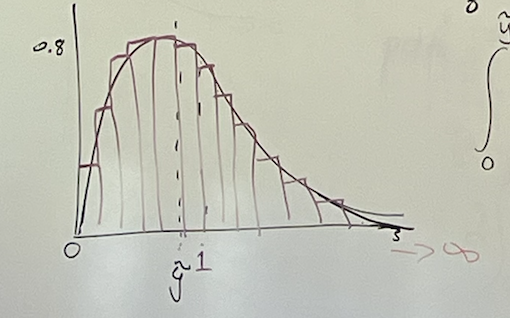
\includegraphics[width=0.5\textwidth]{Screen Shot 2023-10-09 at 11.11.30 AM.png}
    \caption{Histograph}
    % \label{fig:sample}
\end{figure}

\subsection{Mean}
To find a mean, we sum the values and divide it by the number of people we summed over. This is the same as multiplying everyone's value by $\frac{1}{N}$. 
\begin{align}
   E[Y]= \bar y &= \frac{1}{N}\sum_n y_n\\
   &= \sum_n \frac{1}{N} y_n
\end{align}


We can use the pdf to get our mean! The pdf would replace the $\frac{1}{N}$ and the sum would be replaced by the integral. 

\begin{align}
    E[Y]= \bar y = \int_0^\infty 2ye^{-y^2} * y dy
\end{align}

Important: I let the pdf be $f(y)$ for the mean and variance examples.
\begin{align}
    f(y) = pdf(y)
\end{align}

The general rule for finding the mean of a random variable by using the pdf $f(y)$ of that random variable is 
\begin{align}
    E[Y] = \int_\Omega y f(y) dy
\end{align}
where $\Omega$ is the support of $y$. \\

\subsection{Function of the random variable}

Now, let's say you're interest in the function of a mean. You're interested in $g(y)$ rather that $y$ itself.
\begin{align}
    E[g(y)] = \int_\Omega g(y) f(y) dy
\end{align}
where $f(y)$ continues to be the pdf of $Y$. This doesn't break jensen's inequality.

\subsection{Variance}
We an use the pdf to find the variance of $Y$, as well.
\begin{align}
        VAR(Y) = \int_\Omega y^2 f(y) dy - E(y)^2
\end{align}

\section{Uniform Distribution Example}
Consider the uniform ditribution's pdf 
\begin{align}
    f(y) = \frac{1}{\theta_2 - \theta_1}
\end{align}
Let $\theta_2 = 1$ and $\theta_1 = 0$

\begin{align}
    f(y) = \frac{1}{1 - 0}\\
    f(y) = 1
\end{align}

Prove $f(y)$ \textbf{is a pdf} by showing it integrates to 1. 
\begin{align}
    \int_0^1 1 dy = y \bigg|_0^1 = 1 - 0 = 1
\end{align}

What's the mean? 
\begin{align}
    E(Y) = \int_0^1 y *1 dy = \frac{1}{2} y^2 \bigg|_0^1 = \frac{1}{2}
\end{align}

What's the median? 
\begin{align}
    Med(Y) = \int_0^{\tilde y} dy = 0.5 \\
    y\bigg|_0^{\tilde y} = 0.5 \\
    \tilde y - 0 = 0.5
\end{align}

What's the variance?
\begin{align}
    Var(Y) &= \int_0^1 y^2 dy - \frac{1}{2}^2\\
    &= \frac{1}{3}y^3 \bigg|_0^1  -  \frac{1}{2}^2  \\
    &= \frac{1}{3} - \frac{1}{4} \\
    &= \frac{1}{12}
\end{align}

\end{document}